\chapter{Experimental Design}
\label{chap:experiments}
\section{Validation Strategy}
The experiments are organized from isolated process validation to full-product integration. The sequence is shown in Fig.~\ref{fig:experimental_sequence}.
\begin{figure}[t]
    \centering
    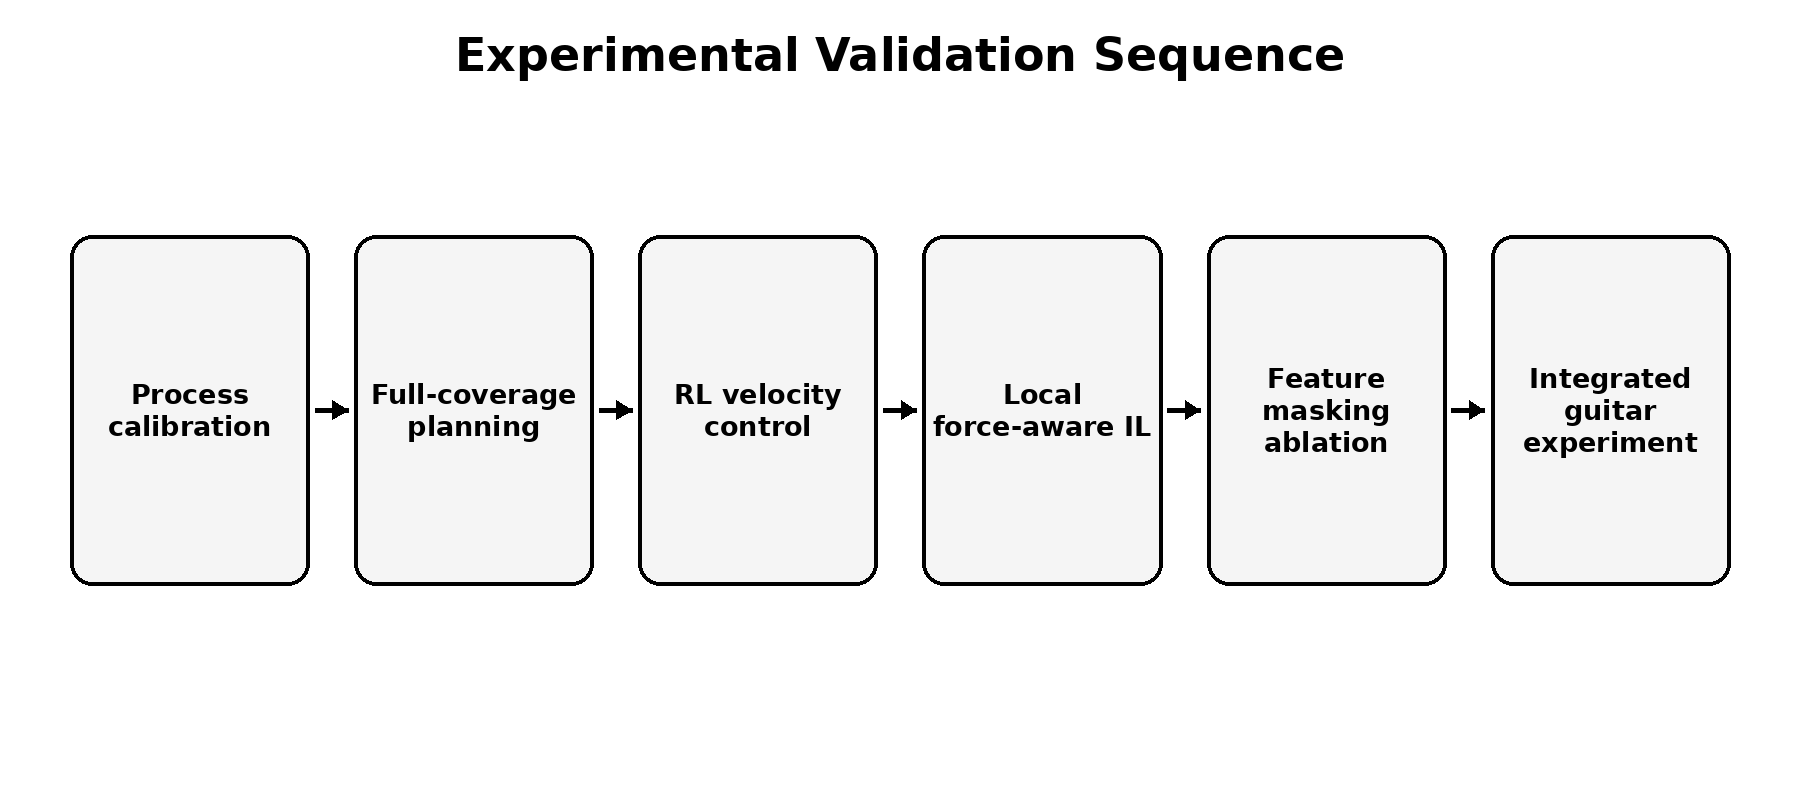
\includegraphics[width=0.98\textwidth]{./7.ExperimentalDesign/figs/experimental_sequence.png}
    \caption{Planned experimental validation sequence.}
    \label{fig:experimental_sequence}
\end{figure}

\section{Hardware and Test Objects}
The target hardware includes a UR10e-class robot, a six-axis force/torque sensor, a polishing spindle, interchangeable broad and local polishing tools, an RGB-D scanner, a local RGB camera, and a rigid guitar fixture. Early tests use coated flat and convex coupons. Geometry experiments use 3-D printed or sacrificial guitar-body replicas before valuable instruments are introduced.

The final object set should contain at least three body classes, for example a double-cut solid body, a single-cut or arched body, and an acoustic or violin-like curved body. Local tests include body edges, cutaways, neck transitions, frets, pickup or bridge regions, and removable metal coupons that reproduce guitar hardware finish.

\section{Process-Model Calibration}
Normal force, sliding velocity, dwell time, tool tilt, spindle speed, pad type, and abrasive compound are varied on coupons. Actual removal is measured using profilometry, thickness change, mass change, or high-resolution surface reconstruction. These tests calibrate the Preston coefficient and the effective contact-footprint model used by Chapters~\ref{chap:full_coverage} and~\ref{chap:rl}.

\section{Full-Coverage Path-Planning Experiments}
The path planner is compared with fixed planar raster motion, nominal-CAD projection, constant-spacing mesh projection, curvature-aware spacing, and the proposed tool-footprint-aware planner. Metrics include target coverage, boundary coverage, over-processed overlap, path length, orientation smoothness, manipulator feasibility, collision clearance, and planning time.

\section{RL Sliding-Velocity Experiments}
The same path and admittance controller are used for fixed speed, inverse-Preston control, PID or model-based rate control, and RL velocity modulation. Tests vary curvature, force bias, sensor delay, friction, pad stiffness, and velocity saturation. Both predicted Preston-rate variation and measured-removal variation are reported.

\section{Force-Aware IL Experiments}
Local tasks are evaluated under unseen geometry, initial pose offset, finish color, reflection, wear or oxidation pattern, friction, pad condition, and contact disturbance. Baselines are manual local programming, RGB-only IL, RGB plus force observation with fixed desired force, and full 9-D pose--force IL. The policy is evaluated on task completion, local coverage, force RMSE, peak force, contact loss, collision, intervention, smoothness, and teaching time.

\section{Feature-Masking Experiments}
Chapter~\ref{chap:feature_masking} is evaluated separately from the core IL policy. Mask quality is varied systematically through boundary erosion, dilation, random holes, delayed updates, and identity errors. Lighting, background, camera pose, and distractors are changed while geometry remains fixed. The study compares raw RGB, static mask conditioning, VIOLA-style region tokens, Mask2Act-style future masks, and the combined model.

\section{Integrated Full-Product Experiment}
The complete experiment performs CAD or scan registration, full-coverage planning, RL speed modulation on broad surfaces, local IL execution at designated regions, and final quality inspection. The integrated framework is compared with geometry-only automation and a semi-automated framework in which a human manually specifies the local paths.

\section{Baselines}
\begin{table}[t]
\centering
\caption{Planned experimental baselines.}
\label{tab:baselines}
\begin{adjustbox}{width=\textwidth}
\begin{tabular}{lll}
\toprule
ID & Method & Purpose \\
\midrule
B0 & Manual expert & Human quality and time reference \\
B1 & Basic CAD coverage + fixed speed & Conventional geometric baseline \\
B2 & Advanced region/contact-point planning & Strong geometry baseline \\
B3 & B2 + manually programmed local paths & Semi-automated baseline \\
B4 & RGB-only IL, 6-D pose, fixed force & Vision-only learning \\
B5 & RGB + wrench observation, fixed force & Force observation only \\
B6 & 9-D pose--force IL & Core local policy \\
B7 & Fixed path speed & Process baseline \\
B8 & Inverse-Preston speed control & Analytical strong baseline \\
B9 & PID/model-based rate control & Feedback strong baseline \\
B10 & RL velocity-scale policy & Proposed process policy \\
B11 & VIOLA-style region tokens & Object-centric masking \\
B12 & Mask2Act-style future masks & Predictive latent plan \\
Full & Global planner + RL + IL + masking & Integrated framework \\
\bottomrule
\end{tabular}
\end{adjustbox}
\end{table}

\section{Evaluation Metrics}
\begin{table}[t]
\centering
\caption{Evaluation metrics.}
\label{tab:metrics}
\begin{adjustbox}{width=\textwidth}
\begin{tabular}{ll}
\toprule
Category & Metrics \\
\midrule
Coverage & Coverage ratio, uncovered area, boundary completion, excessive overlap \\
Removal & Preston-rate CV, cumulative-removal CV, target-band violation, measured removal \\
Surface quality & Roughness, gloss uniformity, residual defect, edge damage \\
Contact & Force RMSE, peak force, $dF/dt$, contact loss, tool-normal error \\
Safety & Collision, near-collision, overload, retraction, intervention \\
Efficiency & Scan, planning, teaching, cycle, and non-processing time \\
Generalization & Geometry, pose, appearance, wear, friction, and pad-condition success \\
\bottomrule
\end{tabular}
\end{adjustbox}
\end{table}

\section{Statistical Analysis}
Each method-condition pair is repeated across multiple specimens and trials. Method and test condition are treated as fixed factors; specimen and guitar model can be treated as random effects in a mixed-effects analysis. Failure modes are categorized as reconstruction error, coverage-planning error, kinematic infeasibility, local-policy perception error, contact instability, termination error, mask error, and out-of-distribution behavior.

\section{Planned and Existing Results}
Only internal simulation results for RL adaptive velocity are currently available. All other numerical results remain planned experiments and must be reported without fabrication. The final thesis should distinguish simulation, coupon, replica, and real-guitar results clearly.
